\section{Introduction}
\subsection{Motivation}
A memorable viewing experience includes the people in the room. Friends may laugh at the same unexpected line, a couple may gasp at a plot twist, or a home party may erupt during a tense scene. These reactions happen without warning. Reaching for a phone after the moment has passed cannot recover the initial reaction, while recording an entire evening leaves users with material to search and edit.

Encore Moment helps viewers preserve these spontaneous moments while remaining engaged with one another and the screen. Friends, couples, families, and party guests may want to revisit a shared response without assigning someone to operate a camera. Streamers and reaction-content creators also need to find spontaneous reactions without reviewing an entire recording. The system identifies candidate moments and describes observable reactions rather than claiming to infer private emotions. Users decide whether a saved moment is suitable to keep or use elsewhere.

\subsection{User and Client Needs}
Viewers need relevant highlights, enough context to remember the scene, and controls that are easy to understand during viewing. A film's laugh track or scream should not be mistaken for a person in the room. Users should know when sensing is active, be able to stop it, and review or delete saved clips. Reaction intensity can help prioritize review, but it cannot determine a person's emotional state or the personal importance of a memory.

The client needs a PC application with a clear feature scope, understandable privacy controls, and explicit support for the demonstration devices and team-controlled player. The application must make sensing status, available highlights, and clip deletion easy to understand.

The demonstration uses a PC, a microphone, an optional webcam, and a player controlled by the team. The player supplies its decoded playback audio, title, position, and play/pause/seek changes. This makes acoustic echo cancellation (AEC) and scene association implementable without assuming access to third-party streaming applications. Saved video depicts the audience. Native TV integration, mobile clients, and recording the viewed program are outside this implementation baseline.

The PC preprocesses audio, manages sensing controls and a disk-based circular video buffer, and creates saved clips. The AWS server performs audio recognition, facial analysis, event fusion, and event-record management. High-quality audience footage stays on the PC; only analysis audio and reduced-resolution camera frames are transmitted. Saved audience clips are stored locally on the PC. Figure~\ref{fig:processing} summarizes this processing boundary. Section~III identifies development baselines that still require integration validation.

\begin{figure*}[!t]
\centering
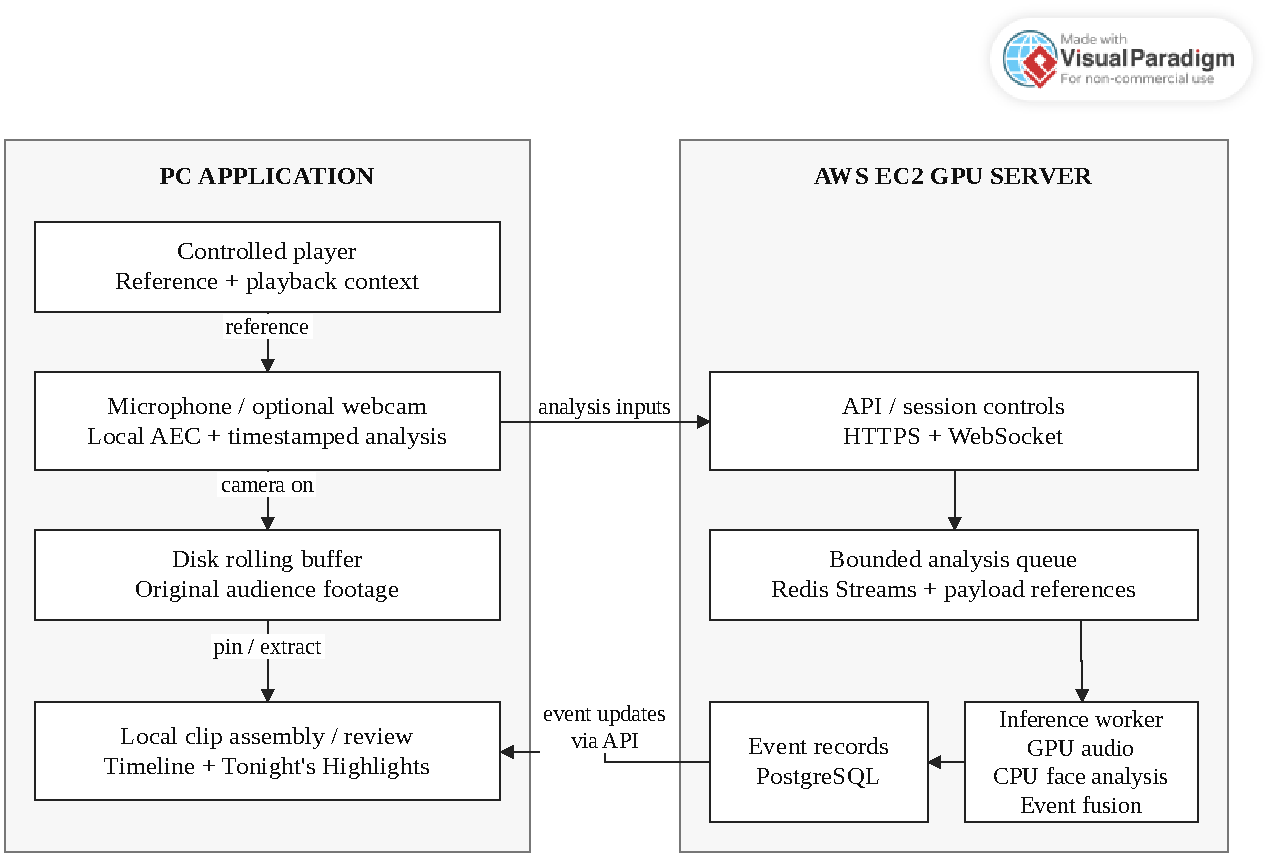
\includegraphics[width=0.88\textwidth]{images/processing-structure.pdf}
\caption{Planned processing structure. The controlled player supplies playback context as well as the AEC reference. Event updates return through the API; continuous original audience footage remains on the PC. Camera-dependent paths are inactive while the camera is off.}
\label{fig:processing}
\end{figure*}

\subsection{Related Software}
\textit{Capture and highlight services.} Reaction-triggered clipping is established in gaming and streaming software. SteelSeries Moments clips laughter and excited vocal reactions detected by the microphone, a feature later named Reaction Clipping~\cite{steel55,steel70}. Twitch Auto Clips creates clips through speech recognition and AI in an invitation-only alpha~\cite{twitch}, and Medal triggers clips from game events~\cite{medal}. OBS Studio exposes replay-buffer operations that illustrate retaining recent media and saving it on demand~\cite{obs}. Encore Moment adds reaction-driven selection, playback context, and sensing controls for shared viewing, where audience reactions must be separated from playback sound.

\textit{Sound event models.} The system will use a pretrained sound-event model such as YAMNet~\cite{yamnet} or PANNs~\cite{panns,pannsweights}. Both are trained on AudioSet, and their labels include laughter, screaming, and gasp. EfficientAT, BEATs, and CLAP remain secondary comparisons for resource use, pretrained representations, and zero-shot audio-text matching~\cite{efficientat,beats,clap}. Speech-emotion models such as audEERING's dimensional model predict arousal, dominance, and valence from podcast speech~\cite{audeering}; that task differs from brief nonverbal reactions, so classifier confidence, acoustic intensity, and emotional significance are kept distinct.

\textit{Facial observations.} MediaPipe Face Landmarker supplies facial landmarks and blendshape observations~\cite{mediapipe}. These can support reaction evidence but do not establish an emotional state or speaker identity.

\textit{Datasets.} FSD50K provides human-labeled laughter, scream, and gasp audio, but its clip-level labels give no precise reaction boundaries or intensity, and individual sound licenses must be checked~\cite{fsd50k}. FSDKaggle2019 has no laughter class and largely overlaps FSD50K~\cite{fsdkaggle,dcase}, so the two are not treated as independent training and evaluation sets. VocalSound adds confusable human sounds such as sighs and coughs but lacks gasp and scream~\cite{vocalsound}. Public data supports initial comparison; consented soundtrack-only, audience-only, and mixed room recordings are still required.

\textit{Echo cancellation and recording.} WebRTC's Audio Processing Module provides playback-reference and microphone interfaces for AEC~\cite{webrtc}, and the Microsoft AEC Challenge supplies data and baselines~\cite{aecchallenge}. Their use in speech applications does not show that nonverbal reactions survive cancellation. GStreamer's WebRTC audio-processing wrapper and segmented recording element provide the initial media building blocks~\cite{gst-aec,gst-ring}. NVIDIA DeepStream Smart Video Record likewise records from cached media before an event, with keyframe-related limits on the clip beginning~\cite{deepstream}.

\textit{TV interfaces.} LG Smart Cam provides camera and microphone hardware for LG TVs~\cite{lgcam}, but public webOS interfaces do not give ordinary applications access to its camera media or to raw playback audio~\cite{lgforum,lgaudio}. Encore Moment is therefore built as a PC application with a team-controlled player.

These sources do not demonstrate the performance of the proposed combined system in our viewing environment.

\subsection{Team Responsibilities and Roles}
Table~\ref{tab:roles} assigns development roles and module ownership; SW denotes software. Soyeon Seol additionally represents the course User role, and Pavel Kim the Customer role. These internal stakeholder roles support review of user and client needs. All members participate in requirement reviews and integration checks.

\begin{table}[!ht]
\caption{Module Ownership and Role Assignments}
\label{tab:roles}
\centering
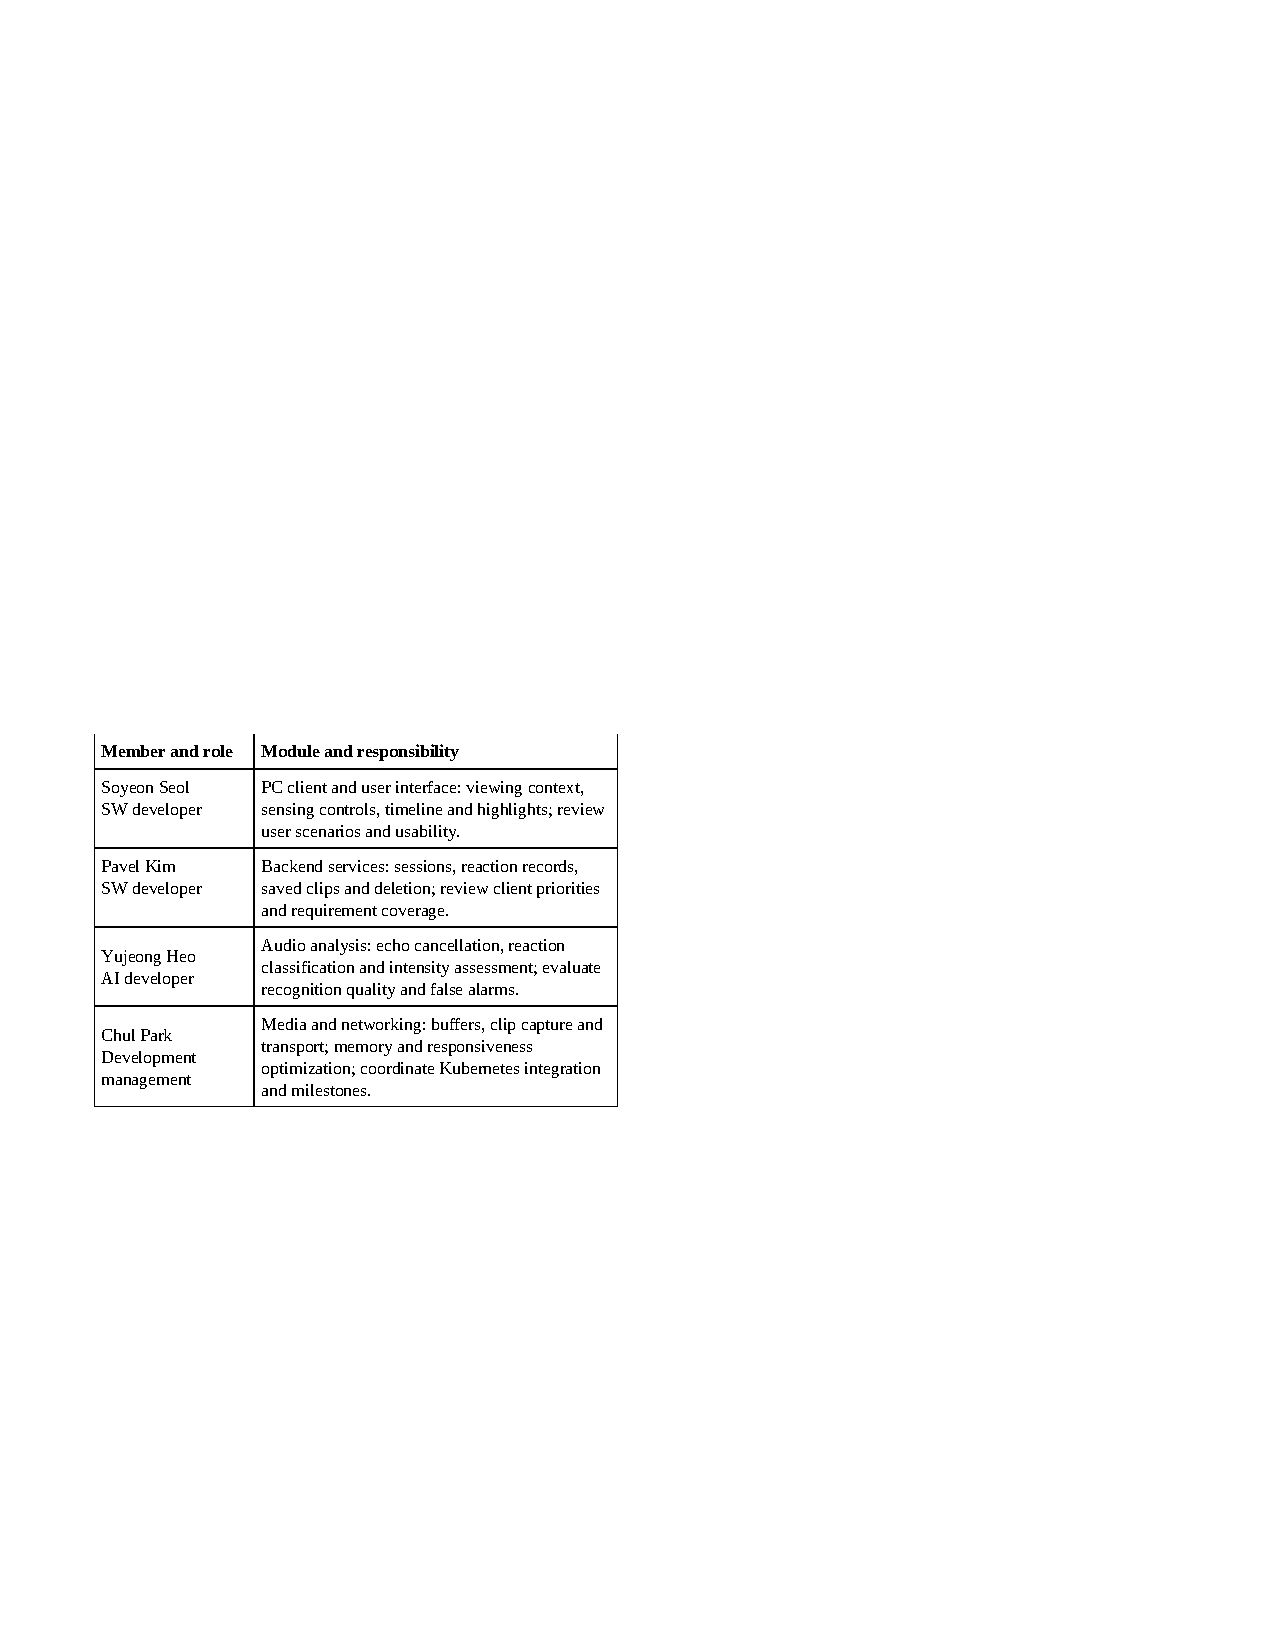
\includegraphics[width=\columnwidth]{images/team-roles.pdf}
\end{table}

This is Submission B, the specification stage of the course project~\cite{assignment}. The repository is \url{https://github.com/SWE-encore/encoremoment}. This document's sources are maintained in \code{submission-b/}. Section~III-C describes the development process and integration responsibilities.
